\documentclass[11pt]{elegantbook}
\definecolor{structurecolor}{RGB}{40,58,129}
\linespread{1.6}
\setlength{\footskip}{20pt}
\setlength{\parindent}{0pt}
\newcommand{\argmax}{\operatornamewithlimits{argmax}}
\newcommand{\argmin}{\operatornamewithlimits{argmin}}
\elegantnewtheorem{proof}{Proof}{}{Proof}
\elegantnewtheorem{claim}{Claim}{prostyle}{Claim}
\DeclareMathOperator{\col}{col}
\title{\textbf{STAT 426}}
\author{Wenxiao Yang}
\institute{Department of Mathematics, University of Illinois at Urbana-Champaign}
\date{}
\setcounter{tocdepth}{2}
\cover{cover.jpg}
\extrainfo{All models are wrong, but some are useful.}

% modify the color in the middle of titlepage
\definecolor{customcolor}{RGB}{32,178,170}
\colorlet{coverlinecolor}{customcolor}
\usepackage{cprotect}

\addbibresource[location=local]{reference.bib} % bib

\begin{document}

\maketitle
\frontmatter
\tableofcontents
\mainmatter

\chapter{Basic of Categorical Data}
\section{Variable Measurement}
\begin{center}\begin{figure}[htbp]
    \centering
    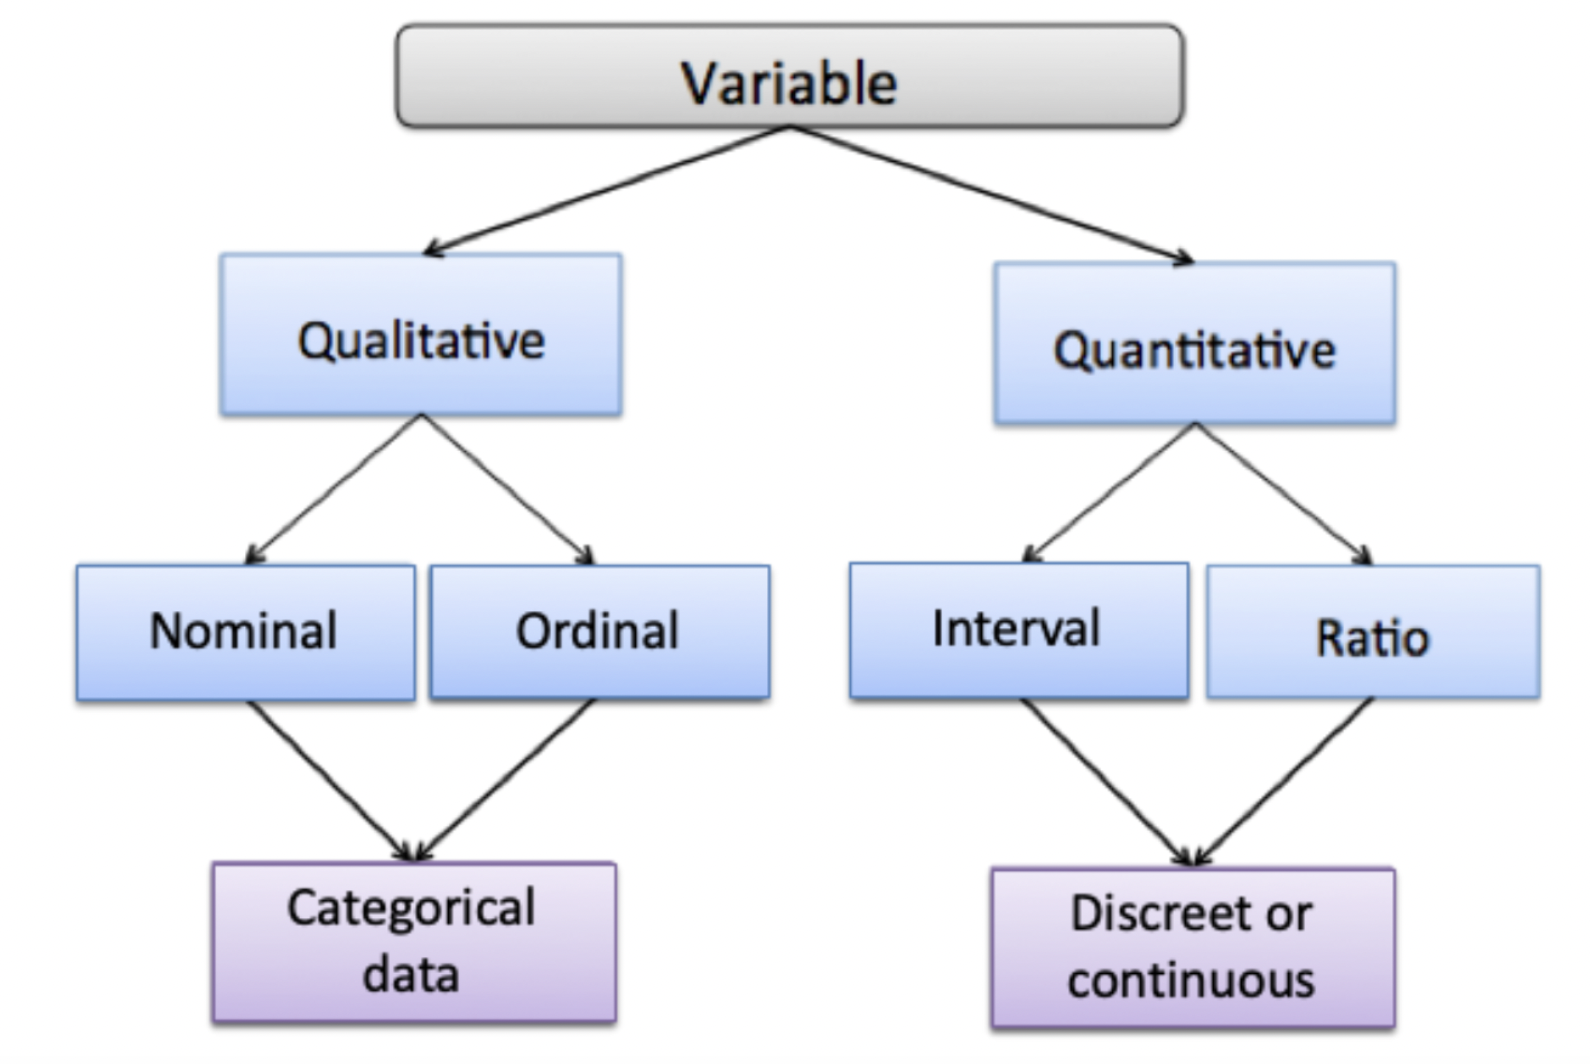
\includegraphics[scale=0.3]{p1.png}
    \caption{Variable Type}
    \label{}
\end{figure}\end{center}
\begin{enumerate}[a)]
    \item Nominal: Categories do not have a natural order. Ex. blood type, gender.
    \item Ordinal: Categories have a natural order. Ex. low/middle/high education level
    \item Interval: There is a numerical distance (difference between two different values is meaningful) between any two values.
    Ex. blood pressure level, 100 blood pressure doesn't mean the double degree of 50 pressure.
    \item Ratio: An interval variable where ratios are valid (presence of absolute zero, i.e. zero is meaningful). Ex. weight, 4g is double degree of 2g, distance run by an athlete.
\end{enumerate}
\subsection*{Levels of measurements}
A variable's level of measurement determines the statistical methods to be used for its analysis.
\begin{center}
    Variables hierarchy: Ratio $>$ Interval $>$ Ordinal $>$ Nominal
\end{center}
Statistical methods applied to variables at a lower level can be used with variables at a higher level, but the contrary is not true.

\section{Statistical Inference for Categorical Data}
There is a distribution $F(\beta)$ with p.d.f. (p.m.f.) $f(x\mid\beta)$, where $\beta$ a generic unknown parameter and $\hat{\beta}$ the parameter estimate.
\subsection{Maximum likelihood Estimation (MLE)}
Given a set of observations $\vec{x}=(x_1,...,x_n)$, the likelihood function of these observations with parameter $\beta$ is $l(\vec{x}\mid\beta)$. We want to find parameter $\hat{\beta}$ that maximizes the likelihood function,$$\hat{\beta}=\arg\max_{\beta} l(\vec{x}\mid\beta)$$
which is also equivalent to maximizing the logarithm of the likelihood function $L(\vec{x}\mid\beta) = \log(l(\vec{x}\mid\beta))$, $$\hat{\beta}=\arg\max_{\beta}L(\vec{x}\mid\beta)$$

\begin{definition}[score function]
    The score function is $$u(\beta,\vec{x})=\nabla_{\beta} L(\vec{x}\mid \beta)=\frac{\nabla_{\beta} l(\vec{x}\mid \beta)}{l(\vec{x}\mid \beta)}$$
\end{definition}
\begin{lemma}[mean of score function]
    The mean of score function is $0$,
    $$\mathbb{E}_{\vec{x}}u(\beta,\vec{x})=0$$
\end{lemma}
\begin{proof}
    \begin{equation}
        \begin{aligned}
            \mathbb{E}_{\vec{x}}u(\beta,\vec{x})&=\int_{\vec{x}}l(\vec{x}\mid \beta)\frac{\nabla_{\beta} l(\vec{x}\mid \beta)}{l(\vec{x}\mid \beta)}d \vec{x}\\
            &=\int_{\vec{x}}\nabla_{\beta} l(\vec{x}\mid \beta)d \vec{x}\\
            &=\nabla_{\beta}\left(\int_{\vec{x}}l(\vec{x}\mid \beta)d \vec{x}\right)\\
            &=\nabla_{\beta}1=0
        \end{aligned}
        \nonumber
    \end{equation}
\end{proof}

\begin{lemma}[variance of score function]
    The variance of the score function is $$\textnormal{Var}_{\vec{x}}(u(\beta, \vec{x}))= \mathbb{E}_{\vec{x}}\left(u(\beta, \vec{x})u(\beta, \vec{x})^T\right)$$
\end{lemma}
\begin{proof}
    Prove by the zero mean.
\end{proof}

\begin{definition}[Fisher information]
    The (Fisher) information is $$\iota(\beta)=-\mathbb{E}_{\vec{x}}\left[\nabla^2_\beta L(\vec{x}\mid\beta)\right]$$
\end{definition}
\begin{lemma}
    The Fisher information is equal to the variance of score function.
    $$\textnormal{Var}_{\vec{x}}(u(\beta, \vec{x}))=\mathbb{E}_{\vec{x}}\left(u(\beta,\vec{x})u(\beta,\vec{x})^T\right)=-\mathbb{E}_{\vec{x}}\left[\nabla^2_\beta L(\vec{x}\mid\beta)\right]=\iota(\beta)$$
\end{lemma}
\begin{proof}
    \begin{equation}
        \begin{aligned}
            \mathbb{E}_{\vec{x}}\left[\nabla^2_\beta L(\vec{x}\mid\beta)\right]=\mathbb{E}_{\vec{x}}\left(\frac{\partial \frac{\nabla_{\beta} l(\vec{x}\mid \beta)}{l(\vec{x}\mid \beta)}}{\partial \beta}\right)=\mathbb{E}_{\vec{x}}\left(\frac{\nabla^2_{\beta} l(\vec{x}\mid \beta)}{l(\vec{x}\mid \beta)}-\frac{\nabla_{\beta} l(\vec{x}\mid \beta)\nabla_{\beta} l(\vec{x}\mid \beta)^T}{(l(\vec{x}\mid \beta))^2} \right)
        \end{aligned}
        \nonumber
    \end{equation}
    where $\mathbb{E}_{\vec{x}}\left(\frac{\nabla^2_{\beta} l(\vec{x}\mid \beta)}{l(\vec{x}\mid \beta)}\right)=\int_{\vec{x}}l(\vec{x}\mid \beta)\frac{\nabla^2_{\beta} l(\vec{x}\mid \beta)}{l(\vec{x}\mid \beta)}d \vec{x}=\int_{\vec{x}}\nabla^2_{\beta} l(\vec{x}\mid \beta)d \vec{x}=\nabla^2_{\beta}\int_{\vec{x}} l(\vec{x}\mid \beta)d \vec{x}=\nabla^2_{\beta} 1=0$
    Hence, $$\mathbb{E}_{\vec{x}}\left[\nabla^2_\beta L(\vec{x}\mid\beta)\right]=-\mathbb{E}_{\vec{x}}\left(\frac{\nabla_{\beta} l(\vec{x}\mid \beta)\nabla_{\beta} l(\vec{x}\mid \beta)^T}{(l(\vec{x}\mid \beta))^2} \right)=-\mathbb{E}_{\vec{x}}\left(u(\beta,\vec{x})u(\beta,\vec{x})^T\right)$$
\end{proof}

\begin{proposition}
    When the sample $x$ is made up of i.i.d. observations, the covariance matrix of the maximum likelihood estimator $\hat{\beta}$ is approximately equal to the inverse of the information matrix. $$\textnormal{Cov}(\hat{\beta})\approx(\iota(\beta))^{-1}$$
\end{proposition}
Hence, the covariance matrix can be estimated as $(\iota(\hat{\beta}))^{-1}$. Similarly, \textit{SE} is estimated by $\sqrt{(\iota(\hat{\beta}))^{-1}}$.

\subsection{Likelihood Inference (Wald, Likelihood-Ratio, Score)}
We want to test
\begin{equation}
    \begin{aligned}
        H_0:\beta=\beta_0\quad\quad H_\alpha:\beta\neq \beta_0
    \end{aligned}
    \nonumber
\end{equation}
or form a confidence interval (CI) for $\beta$.

\begin{definition}[Wald Test]
    The Wald statistic:
    \begin{equation}
        \begin{aligned}
            z_W=\frac{\hat{\beta}-\beta_0}{SE}=\frac{\hat{\beta}-\beta_0}{\sqrt{(\iota(\hat{\beta}))^{-1}}}
        \end{aligned}
        \nonumber
    \end{equation}
    where $\textit{SE}=\sqrt{(\iota(\hat{\beta}))^{-1}}$.\\
    Usually, as $n \rightarrow \infty$, $z_W \stackrel{d}{\longrightarrow} N(0,1)$ under $H_0:\beta=\beta_0$.
    \begin{enumerate}[(1)]
        \item We reject the $H_0$ if $|z_W|\geq z_{\frac{\alpha}{2}}$ for a \underline{two-sided level $\alpha$ test}.
        \item The \underline{$(1-\alpha)100\%$ Wald (confidence) interval} is $$\{\beta_0:|z_W|=\frac{|\hat{\beta}-\beta_0|}{SE}<z_{\frac{\alpha}{2}}\}=(\hat{\beta}-z_\frac{\alpha}{2}SE,\hat{\beta}+z_\frac{\alpha}{2}SE)$$
        \item The Wald test also has a \underline{chi-squared form}, using
        \begin{equation}
            \begin{aligned}
                z_W^2=\frac{(\hat{\beta}-\beta_0)^2}{(\iota(\hat{\beta}))^{-1}}\sim \chi_1^2\quad \textnormal{(under $H_0$)}
            \end{aligned}
            \nonumber
        \end{equation}
    \end{enumerate}
\end{definition}

\begin{definition}[Likelihood Ratio Test]
    Let $$\Lambda=\frac{l(\vec{x}\mid\beta_0)}{l(\vec{x}\mid\hat{\beta})}$$
    where $l(\vec{x}\mid\hat{\beta})=\max_{\beta}l(\vec{x}\mid\beta)$, so the ratio $\Lambda\in [0,1]$.\\
    The \textbf{likelihood-ratio test (LRT) chi-squared statistic}:
    \begin{equation}
        \begin{aligned}
            -2\ln\Lambda=-2\left(L(\beta_0)-L(\hat{\beta})\right)
        \end{aligned}
        \nonumber
    \end{equation}
    It has an approximate $\chi_1^2$ distribution under $H_0 : \beta = \beta_0$, and otherwise tends to be larger.
    \begin{enumerate}[(1)]
        \item Thus, reject $H_0$ if $$-2\ln\Lambda\geq\chi_1^2(\alpha)$$
        \item The \underline{$(1-\alpha)100\%$ likelihood-ratio (confidence) interval} is $$\{\beta_0:-2\ln\Lambda=-2\left(L(\beta_0)-L(\hat{\beta})\right)<\chi_1^2(\alpha)\}$$
        Unlike Wald, this interval is \underline{not degenerate}. (i.e., For general case, the interval does not have an explicit form.)
    \end{enumerate}
\end{definition}

\begin{definition}[Score Test]
    The \textbf{score statistic}: $$z_S=\frac{u(\beta_0)}{\sqrt{\iota(\beta_0)}}$$
    As $n \rightarrow \infty$, $z_S \stackrel{d}{\longrightarrow} N(0,1)$ under $H_0:\beta=\beta_0$. Otherwise, it tends to be further from zero.
    \begin{enumerate}[(1)]
        \item Thus, reject $H_0$ if $|z_S|\geq z_{\frac{\alpha}{2}}$ for a \underline{two-sided level $\alpha$ test}.
        \item The \underline{$(1-\alpha)100\%$ score (confidence) interval} is $$\{\beta_0:|z_S|=\frac{|u(\beta_0)|}{\sqrt{\iota(\beta_0)}}<z_{\frac{\alpha}{2}}\}$$
        Unlike Wald, it is \underline{not degenerate} for some distributions.
        \item There is also a chi-squared form:
        \begin{equation}
            \begin{aligned}
                z_S^2=\frac{u(\beta_0)^2}{\iota(\beta_0)}\sim \chi_1^2\quad \textnormal{(under $H_0$)}
            \end{aligned}
            \nonumber
        \end{equation}
    \end{enumerate}
\end{definition}
We can also use P-value to measure the probability of the statistic is more extreme under the $H_0$. We can reject $H_0$ if the P-value is $\leq\alpha$.

All three kinds tend to be “asymptotically equivalent” as $n \rightarrow \infty$. For smaller $n$, the \underline{likelihood-ratio} and \underline{score} methods are preferred.

\chapter{Association in Contingency Tables}
\section{Association in Two-Way Contingency Tables}
Consider joint observations of two categorical variables: $X$ with $I$ categories, $Y$ with $J$ categories.

We can summarize data in an $I \times J$ \textbf{contingency table}:
\begin{table}[htbp]
    \centering
    \begin{tabular}{lllll}
        &&&$Y$&\\
        &&1&$\cdots$&J\\
        \cline{3-5}
        & \multicolumn{1}{l|}{$1$} & \multicolumn{1}{l|}{} & \multicolumn{1}{l|}{} & \multicolumn{1}{l|}{} \\
        \cline{3-5}
        $X$ &\multicolumn{1}{l|}{$\vdots$}  & \multicolumn{1}{l|}{} & \multicolumn{1}{l|}{} & \multicolumn{1}{l|}{} \\ \cline{3-5}
        & \multicolumn{1}{l|}{$I$} & \multicolumn{1}{l|}{} & \multicolumn{1}{l|}{} & \multicolumn{1}{l|}{} \\ \cline{3-5}
    \end{tabular}
\end{table}\\
Each \textbf{cell} contains a count $n_{ij}$.

\subsection{Distribution}
If both $X$ and $Y$ are random, let $$\pi_{ij}=P(X\text{ in row }i, Y\text{ in col }j)$$
be the \textbf{joint} distribution of $X$ and $Y$.

The \textbf{marginal} distribution of $X$ is defined by $$\pi_{i+}=P(X\text{ in row }i)$$
and similarly for $Y$:
$$\pi_{+j}=P(Y\text{ in col }j)$$

The \textbf{conditional} distribution of $Y$ given that $X$ is in row $i$ is defined by
$$\pi_{j\mid i}=P(Y\text{ in col }j\mid X\text{ in row }i)=\frac{\pi_{ij}}{\pi_{i+}}$$

\subsection{Descriptive Statistics}
Let $n_{ij}=\textit{count in row $i$ and col $j$}$ and $n=\sum_i\sum_jn_{ij}$.\\
The \textbf{margins} of the table:
$$n_{i+}=\sum_jn_{ij},\quad n_{+j}=\sum_in_{ij}$$
\subsubsection*{Natural Estimation}
\begin{enumerate}
    \item Natural estimate of $\pi_{ij}$: $\hat{\pi}_{ij}=\frac{n_{ij}}{n}$
    \item Similarly marginals: $\hat{\pi}_{i+}=\sum_j \hat{\pi}_{ij}=\frac{n_{i+}}{n};\ \hat{\pi}_{+j}=\sum_i p_{ij}=\frac{n_{+j}}{n}$
    \item And conditionals: $\hat{\pi}_{j\mid i}=\frac{\hat{\pi}_{ij}}{\hat{\pi}_{i+}}=\frac{n_{ij}}{n_{i+}}$
\end{enumerate}

\subsection{Sampling Models (Examples)}
Possible joint distributions for counts in $I \times J$ table:
\begin{enumerate}
    \item \underline{Poisson (random total)}: $Y_{ij} =\text{count in cell } (i,j)$,
    $$Y_{ij}\sim \text{Poisson}(\mu_{ij})$$
    and the $Y_{ij}$s are independent.
    \item \underline{Multinomial (fixed total $n$):} $N_{ij} = \text{count in cell } (i,j)$, $$\{N_{ij}\}\sim \text{multinomial}(n,\{\pi_{ij}\})$$
    \item \underline{Independent Multinomial}: Assume $n_{i+}$ (row totals $n_i$) are fixed,
    \begin{equation}
        \begin{aligned}
            \left.\begin{matrix}
                \{N_{1j}\}_{j=1}^J\sim \text{multinomial}(n_1,\{\pi_{j\mid 1}\}_{j=1}^J)\\
                \vdots\\
                \{N_{Ij}\}_{j=1}^J\sim \text{multinomial}(n_I,\{\pi_{j\mid I}\}_{j=1}^J)\\
            \end{matrix}\right\}
        \end{aligned}
        \nonumber
    \end{equation}
    (When $J = 2$, this is \underline{independent binomial sampling}, for which we may just write $\pi_i$ for $\{\pi_{1\mid i},\pi_{2\mid i}\}$.)
\end{enumerate}


\subsection{Independent / Homogeneity}
\begin{definition}[independent]
    If both $X$ and $Y$ are \underline{random}, they are \textbf{independent} if $$\pi_{ij}=\pi_{i+}\pi_{+j},\ \forall i,j$$
    which implies $\pi_{j\mid i}=\frac{\pi_{i+}\pi_{+j}}{\pi_{i+}}=\pi_{+j},\forall i,j$. That is, $\pi_{j\mid i}$ doesn't depend on $i$ and is the same as the marginal distribution of $Y$. (Intuitively, knowing $X$ tells nothing about $Y$.)
\end{definition}
\begin{definition}[homogeneity]
    Even if $X$ is \underline{not really random}, the condition that $\pi_{j\mid i}=\pi_{+j},\forall i,j$ is called \textbf{homogeneity}. This might still be relevant in a situation where $X$ is deliberately chosen and $Y$ is observed as a response.
\end{definition}



\subsection{Measuring Inhomogeneity}
\begin{table}[htbp]
    \centering
    \begin{tabular}{rllll}
        \cline{2-5}
        \multicolumn{1}{r|}{\multirow{2}{*}{}} & \multicolumn{2}{l|}{$n_{11}$} & \multicolumn{2}{l|}{$n_{12}$} \\ \cline{2-5} 
        \multicolumn{1}{r|}{}                   & \multicolumn{2}{l|}{$n_{21}$} & \multicolumn{2}{l|}{$n_{22}$} \\ \cline{2-5}
        \multicolumn{1}{l}{}                    &             &             &             &
    \end{tabular}\\
    \begin{tabular}{rllll}
        \cline{2-5}
        \multicolumn{1}{r|}{\multirow{2}{*}{}} & \multicolumn{2}{l|}{$Y_1$} & \multicolumn{2}{l|}{$n_1-Y_1$} \\ \cline{2-5} 
        \multicolumn{1}{r|}{}                   & \multicolumn{2}{l|}{$Y_2$} & \multicolumn{2}{l|}{$n_2-Y_2$} \\ \cline{2-5}
        \multicolumn{1}{l}{}                    &             &             &             &
    \end{tabular}\\
    where $Y_i\sim$ indep. binomial$(n_i,\pi_i)$. This regards row totals as fixed.
\end{table}
Homogeneity is the condition $\pi_1 = \pi_2$. We can measure inhomogeneity by three different measures:
\begin{enumerate}
    \item \textbf{difference of proportions}: $$\pi_1-\pi_2$$
    The estimation is $$\hat{\pi}_1-\hat{\pi}_2=\frac{y_1}{n_1}-\frac{y_2}{n_2}$$
    The approx $(1-\alpha)100\%$ confidence interval is:
    \begin{equation}
        \begin{aligned}
            \hat{\pi}_1-\hat{\pi}_2\pm z_{\frac{\alpha}{2}}\sqrt{\frac{\hat{\pi}_1(1-\hat{\pi}_1)}{n_1}+\frac{\hat{\pi}_2(1-\hat{\pi}_2)}{n_2}}
        \end{aligned}
        \nonumber
    \end{equation}
    (Problematic if $\pi_1$ and $\pi_2$ are near $0$ or $1$.)
    \item \textbf{relative risk}: $$RR=\frac{\pi_1}{\pi_2}$$
    The estimation is $$r=\frac{\hat{\pi}_1}{\hat{\pi}_2}=\frac{y_1/n_1}{y_2/n_2}$$
    The approx $(1-\alpha)100\%$ confidence interval of $\ln RR$ is:
    \begin{equation}
        \begin{aligned}
            \ln r\pm z_{\frac{\alpha}{2}}\sqrt{\frac{1-\hat{\pi}_1}{y_1}+\frac{1-\hat{\pi}_2}{y_2}}
        \end{aligned}
        \nonumber
    \end{equation}
    \item \textbf{odds ratio}: $$\theta=\frac{\pi_1/(1-\pi_1)}{\pi_2/(1-\pi_2)}$$
    When $\theta=1$, we can say there is no association.\\
    The \textbf{odds} for a probability $\pi$ is $\Omega=\frac{\pi}{1-\pi}$. Note $\pi=\frac{\Omega}{1+\Omega}$.\\
    (In the multinomial model: $\theta=\frac{\pi_{11}\pi_{22}}{\pi_{12}\pi_{21}}$ ("cross-product ratio"); in Poisson model: $\theta=\frac{\mu_{11}\mu_{22}}{\mu_{12}\mu_{21}}$)\\
    The usual (unrestricted) estimates $$\hat{\theta}=\frac{n_{11}n_{22}}{n_{12}n_{21}}$$
    The approx $(1-\alpha)100\%$ confidence interval for $\ln\theta$ is
    \begin{equation}
        \begin{aligned}
            \ln\hat{\theta}\pm z_{\frac{\alpha}{2}}\sqrt{\frac{1}{n_{11}}+\frac{1}{n_{12}}+\frac{1}{n_{21}}+\frac{1}{n_{22}}}
        \end{aligned}
        \nonumber
    \end{equation}
    Useful properties of odds ratio:
    \begin{enumerate}[(1)]
        \item Interchanging rows (or cols) changes $\theta$ to $\frac{1}{\theta}$.
        \item Interchanging $X$ and $Y$ doesn't change $\theta$.
        \item Multiplying a row (or col) by a factor doesn't change $\hat{\theta}$.
        \item Relationship to relative risk: $\theta=RR\cdot\frac{1-\pi_2}{1-\pi_1}$. ($\theta$ and $RR$ are similar if both $\pi_1$ and $\pi_2$ are small.)
    \end{enumerate}
\end{enumerate}
\subsection{Delta Method}
It is easy to obtain approximate CI for a mean based on a sample mean by using the Central Limit Theorem and a consistent estimate of standard error.

But the log Odds Ratio and log Relative Risk are transformed means. How were their CI's derived? And why take logs?

Suppose a statistic $T_n$ and parameter $\theta$ such that
$$
\sqrt{n}\left(T_n-\theta\right) \underset{n \rightarrow \infty}{\stackrel{d}{\longrightarrow}} N\left(0, \sigma^2\right)
$$
(e.g. $T_n$ might be a sample mean from a sample of size $n$ with population mean $\theta$ and variance $\sigma^2$)

We want a CI for $g(\theta)$, for some smooth $g$.

The Taylor expand at $T_n$ is
\begin{equation}
    \begin{aligned}
        %g(T_n)\approx g(\theta)+g'(\theta)(T_n-\theta)
        g(\theta)\approx g(T_n)+g'(T_n)(\theta-T_n)
    \end{aligned}
    \nonumber
\end{equation}
So,
\begin{equation}
    \begin{aligned}
        \sqrt{n}(g(T_n)-g(\theta))\approx g'(T_n)\sqrt{n}(T_n-\theta)\underset{n \rightarrow \infty}{\stackrel{d}{\longrightarrow}} N\left(0, (g'(T_n))^2\sigma^2\right)
    \end{aligned}
    \nonumber
\end{equation}
(This is useful only if $g'(T_n)\neq 0$)
Hence, when $n$ is large
\begin{equation}
    \begin{aligned}
        \sqrt{n}\frac{g(T_n)-g(\theta)}{|g'(T_n)|\sigma} \quad \dot{\sim}\quad  N(0,1)
    \end{aligned}
    \nonumber
\end{equation}
which suggests this approximate CI for $g(\theta)$:
\begin{equation}
    \begin{aligned}
        g(T_n)\pm z_{\frac{\alpha}{2}}\frac{|g'(T_n)|\sigma}{\sqrt{n}}
    \end{aligned}
    \nonumber
\end{equation}



\subsection{Testing Independence: $X^2$ and $G^2$ Test}
Let $\mu_{ij}=\mathbb{E}(N_{ij})=n\pi_{ij}$. Under $H_0:\pi_{ij}=\pi_{i+}\pi_{+j},\ \forall i,j$
\begin{equation}
    \begin{aligned}
        \mu_{ij}=n\pi_{ij}=n\pi_{i+}\pi_{+j}
    \end{aligned}
    \nonumber
\end{equation}
Under $H_0$, can show the MLEs are
\begin{equation}
    \begin{aligned}
        \hat{\mu}_{ij}=n\hat{\pi}_{i+}\hat{\pi}_{+j}=n\left(\frac{n_{i+}}{n}\right)\left(\frac{n_{+j}}{n}\right)=\frac{n_{i+}n_{+j}}{n}
    \end{aligned}
    \nonumber
\end{equation}
(assuming no empty rows or cols)\\
\textbf{Residuals:}
\begin{enumerate}
    \item Raw: $n_{ij}-\hat{\mu}_{ij}$
    \item Pearson: $e_{ij}=\frac{n_{ij}-\hat{\mu}_{ij}}{\sqrt{\hat{\mu}_{ij}}}$. $X^2=\sum_i\sum_j e_{ij}^2$.
    \item Standardized: $r_{ij}=\frac{n_{ij}-\hat{\mu}_{ij}}{\sqrt{\hat{\mu}_{ij}(1-\hat{\pi}_{i+})(1-\hat{\pi}_{+j})}}$
\end{enumerate}
\textbf{Usage:} Look for Pearson or standardized residuals with absolute value \textit{exceeding 2 or 3}. These suggest the reason for significant dependence.

\textbf{Remark:} Under independence, both Pearson and standardized residuals are asymp. normal, but only standardized has asymp. variance equal to 1.

\begin{definition}[$X^2$ Test: Pearson $\chi^2$ Test (Score Test)]
    $$X^2=\sum_{i j} \frac{\left(n_{i j}-\hat{\mu}_{i j}\right)^2}{\hat{\mu}_{i j}} \quad \underset{H_0}{\dot{\sim}}\quad \chi_{(I-1)(J-1)}^2$$
    Note:
    $$
    \begin{aligned}
    (I-1)(J-1) & =(I J-1)-((I-1)+(J-1)) \\
    & =\text { total \# params. }-\# \text { params. under } H_0
    \end{aligned}
    $$
    Reject $H_0$ if
    $$
    X^2>\chi_{(I-1)(J-1)}^2(\alpha)
    $$
    (or use $P$-value)
\end{definition}

\begin{definition}[$G^2$ Test: Likelihood Ratio $\chi^2$ Test]
    $$G^2=2\sum_{i j}n_{ij} \ln \frac{n_{i j}}{\hat{\mu}_{i j}} \quad \underset{H_0}{\dot{\sim}}\quad \chi_{(I-1)(J-1)}^2$$
    Reject $H_0$ if
    $$G^2>\chi_{(I-1)(J-1)}^2(\alpha)$$
    (or use $P$-value)\\
    (Convention: $0 \ln 0 = 0$)
\end{definition}
\textbf{Comparison:}
\begin{enumerate}
    \item $X^2$ and $G^2$ are asymptotically equivalent under $H_0$
    \item The $X^2$ tends to be better.
\end{enumerate}
\begin{example}
    Testing independence is equivalent to testing homogeneity in the indep. binomial model:
    $$
    H_0: \pi_1=\pi_2
    $$
    Can show
    $$
    X^2=z^2
    $$
    where
    $$
    z=\frac{\hat{\pi}_1-\hat{\pi}_2}{\sqrt{\hat{\pi}(1-\hat{\pi})\left(1 / n_1+1 / n_2\right)}} \quad \hat{\pi}=\frac{y_1+y_2}{n_1+n_2}
    $$
\end{example}
\textbf{Remark:} The $X^2$ and $G^2$ tests are not necessarily compatible with the Wald CIs. For example,
\begin{center}
    reject $H_0$ $\nLeftrightarrow$  odds ratio $\theta =\frac{\pi_1/(1-\pi_1)}{\pi_2/(1-\pi_2)}= 1$ not in Wald CI
\end{center}

\subsection{Testing Independence: Fisher's Exact Test}
When cell counts are small, the $X^2$ and $G^2$ independence tests are not recommended: The $\chi^2$ approximations are poor. In this section we introduce a \textit{Fisher's Exact Test}.

Consider a $2 \times 2$ table with row and col totals fixed:
$$
\begin{array}{c|c|c|c}
\multicolumn{3}{c}{Y} \\
\cline { 2 - 3 } X & N_{11} & N_{12} & n_{1+} \\
\cline { 2 - 3 } & N_{21} & N_{22} & n_{2+} \\
\cline { 2 - 3 } \multicolumn{1}{c}{}&\multicolumn{1}{c}{n_{+1}}&\multicolumn{1}{c}{n_{+2}}&\multicolumn{1}{c}{n}
\end{array}
$$
\textbf{Note:} \underline{Any cell count, say $N_{11}$, determines the whole table.}

Can show that, under $H_0$ : independence, $N_{11}$ is (conditionally) hypergeometric:
$$
\mathrm{P}_{H_0}\left(N_{11}=t\right)=\frac{\begin{pmatrix}
    n_{1+} \\
    t
\end{pmatrix}\begin{pmatrix}
    n_{2+}\\
    n_{+1}-t
\end{pmatrix}}{\begin{pmatrix}
    n \\
    n_{+1}
\end{pmatrix}}
$$
In terms of odds ratio $\theta=\frac{\pi_1/(1-\pi_1)}{\pi_2/(1-\pi_2)}$, independence is $$H_0:\theta=1$$
Possible alternatives:
\begin{equation}
    \begin{aligned}
        H_\alpha:\theta>1 \quad &\Rightarrow\quad N_{11} \textnormal{ tends larger}\\
        H_\alpha:\theta<1 \quad &\Rightarrow\quad N_{11} \textnormal{ tends smaller}\\
        H_\alpha:\theta\neq 1 \quad &\Rightarrow\quad N_{11} \textnormal{ tends larger or smaller}
    \end{aligned}
    \nonumber
\end{equation}
For $H_\alpha:\theta>1$, the (one-sided) $p$-value is $\mathrm{P}_{H_0}\left(N_{11}\geq t_0\right)$, where $t_0=n_{11}$ is the observed value of $N_{11}$.

\textbf{Remarks:} Could use mid $p$-values instead; Implemented in R function fisher.test(); Can be extended to $I \times J$ tables (with some computational difficulty).


\section{Conditional Association in Three-Way Tables}
Add a third categorical variable $Z$.
\begin{example}
    Is a drug more effective at curing a disease among younger patients than among older?
    $X=$ drug or placebo; $Y=$ disease cured or not; $Z=$ age group (young, old).
\end{example}
\subsection{Conditional Association}
$Z$ may be called a \textbf{stratification variable}. We are interested in the distribution of $(X, Y)$ \textit{conditional} on $Z$.

\begin{definition}[partial table]
    Each $Z$ category defines a \textbf{partial table} for $X$ and $Y$.
\end{definition}
\begin{example}
    When $Z = 1, 2$ and $X , Y$ are binary ($2\times 2 \times 2$ table):
    \begin{table}[htbp]
        \centering
        $Z=1:$
        \begin{tabular}{rllll}
            \multicolumn{1}{c}{}                    & \multicolumn{4}{c}{$Y$}                                 \\ \cline{2-5} 
            \multicolumn{1}{r|}{\multirow{2}{*}{$X$}} & \multicolumn{2}{l|}{$n_{111}$} & \multicolumn{2}{l|}{$n_{121}$} \\ \cline{2-5} 
            \multicolumn{1}{r|}{}                   & \multicolumn{2}{l|}{$n_{211}$} & \multicolumn{2}{l|}{$n_{221}$} \\ \cline{2-5}
            \multicolumn{1}{l}{}                    &             &             &             &
        \end{tabular}\quad\quad
        $Z=2:$
        \begin{tabular}{rllll}
            \multicolumn{1}{c}{}                    & \multicolumn{4}{c}{$Y$}                                 \\ \cline{2-5} 
            \multicolumn{1}{r|}{\multirow{2}{*}{$X$}} & \multicolumn{2}{l|}{$n_{112}$} & \multicolumn{2}{l|}{$n_{122}$} \\ \cline{2-5} 
            \multicolumn{1}{r|}{}                   & \multicolumn{2}{l|}{$n_{212}$} & \multicolumn{2}{l|}{$n_{222}$} \\ \cline{2-5}
            \multicolumn{1}{l}{}                    &             &             &             &
        \end{tabular}\\
        These represent \textbf{conditional associations}.
    \end{table}\\
\end{example}

\begin{definition}[marginal table]
    The \textbf{marginal table} sums the partial tables:
\end{definition}
\begin{table}[htbp]
    \centering
    \begin{tabular}{rllll}
        \multicolumn{1}{c}{}                    & \multicolumn{4}{c}{$Y$}                                 \\ \cline{2-5} 
        \multicolumn{1}{r|}{\multirow{2}{*}{$X$}} & \multicolumn{2}{l|}{$n_{11+}$} & \multicolumn{2}{l|}{$n_{12+}$} \\ \cline{2-5} 
        \multicolumn{1}{r|}{}                   & \multicolumn{2}{l|}{$n_{21+}$} & \multicolumn{2}{l|}{$n_{22+}$} \\ \cline{2-5}
        \multicolumn{1}{l}{}                    &             &             &             &
    \end{tabular}\\
    This represents the \textbf{marginal association} (ignoring $Z$).
\end{table}
In general, let $\mu_{ijk}=\textit{ expected count in row i, col j, table k}$.\\
The \textbf{conditional odds ratios},
\begin{equation}
    \begin{aligned}
        \theta_{XY(k)}=\frac{\mu_{11k}\mu_{22k}}{\mu_{12k}\mu_{21k}}
    \end{aligned}
    \nonumber
\end{equation}
which are estimated by
\begin{equation}
    \begin{aligned}
        \hat{\theta}_{XY(k)}=\frac{n_{11k}n_{22k}}{n_{12k}n_{21k}}
    \end{aligned}
    \nonumber
\end{equation}
The \textbf{marginal odds ratio}
\begin{equation}
    \begin{aligned}
        \theta_{XY}=\frac{\mu_{11+}\mu_{22+}}{\mu_{12+}\mu_{21+}}
    \end{aligned}
    \nonumber
\end{equation}
is estimated from the marginal table.

\subsection{Simpson's Paradox}
Some counter-intuitive but possible situations:
\begin{enumerate}
    \item There are conditional associations ($\theta_{XY(k)} \neq 1$) but no marginal
    association ($\theta_{XY} = 1$)
    \item There is a marginal association ($\theta_{XY} \neq 1$) but no conditional associations ($\theta_{XY(k)} = 1$)
    \item \textbf{Simpson's paradox}: The conditional associations are in the opposite direction from the marginal, e.g. $\theta_{XY(k)}>1,\theta_{XY}<1$
    \begin{center}\begin{figure}[htbp]
        \centering
        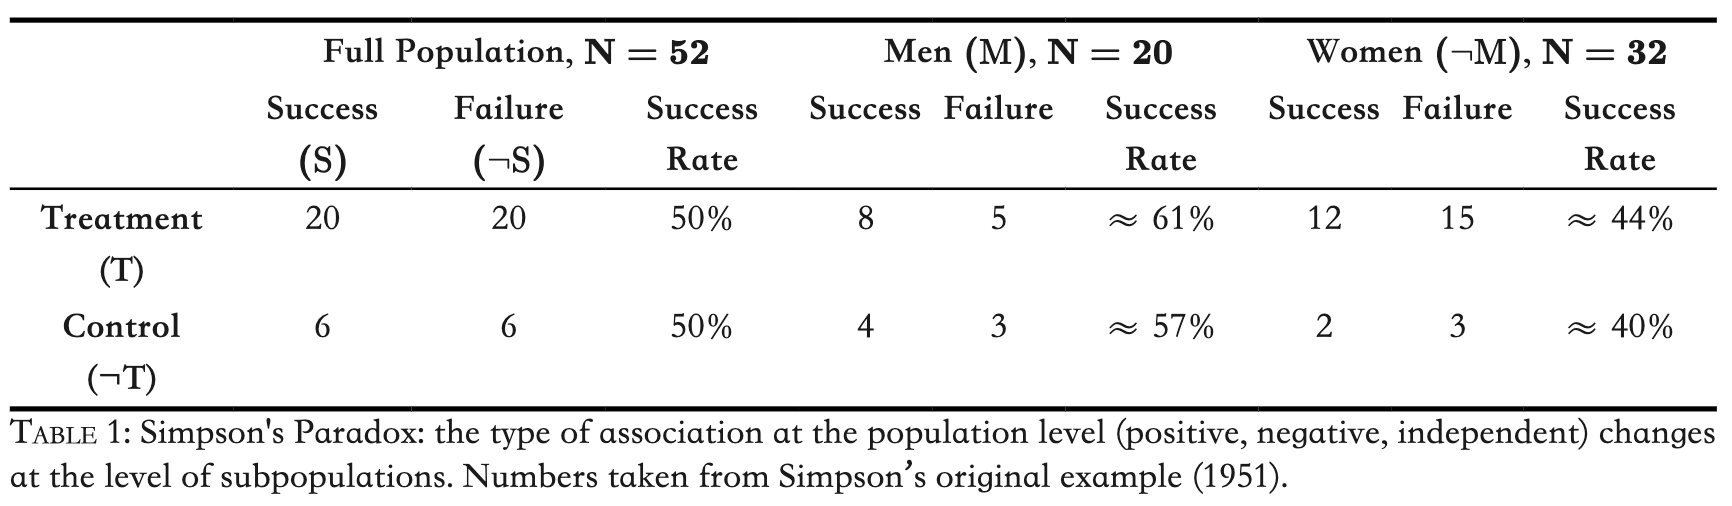
\includegraphics[scale=0.2]{Simpson's Paradox.png}
        \caption{Simpson's paradox}
        \label{}
    \end{figure}\end{center}
\end{enumerate}

\subsection{Conditional Independence, Marginal Independence}
\begin{definition}[conditionally independent given $Z$, marginal independent]
    We also call $X$ and $Y$ are \textbf{conditionally independent given $Z = k$} if $\theta_{XY(k)}=1$. If this is true for all $k$, $X$ and $Y$ are \textbf{conditionally independent given $Z$}. Not the same to "$X$ and $Y$ are \textbf{marginal independent} if $\theta_{XY}=1$".
\end{definition}

\begin{proposition}
    For \underline{multinomial sampling}, can show that conditional independence is
    \begin{equation}
        \begin{aligned}
            \pi_{ijk}=\frac{\pi_{i+k}\pi_{+jk}}{\pi_{++k}},\quad \forall i,j,k
        \end{aligned}
        \nonumber
    \end{equation}
\end{proposition}

\subsection{Homogeneous Association}
\begin{definition}
    Let $Z$ have $K$ categories. $X$ and $Y$ have \textbf{homogeneous association} over $Z$ if
    \begin{equation}
        \begin{aligned}
            \theta_{XY(1)}=\theta_{XY(2)}=\cdots=\theta_{XY(K)}
        \end{aligned}
        \nonumber
    \end{equation}
    (Conditional independence is a special case.)
\end{definition}

\chapter{Generalized Linear Models}
\section{Introduction}
A linear model $Y=\alpha+\sum_{i=1}^p \beta_i x_i +\varepsilon$ is usually not appropriate if $Y$ is binary or a count.

\subsection{Definition}
We seek to model independent observations $Y_1,...,Y_n$ of a \textbf{response variable}, in terms of corresponding vectors $\vec{x}_i=(x_{i1},...,x_{ip}),i=1,...,n$ of values of $p$ \textbf{explanatory variables}.

\begin{enumerate}[(1)]
    \item \textbf{\underline{Random component:}} density of $Y_i$ from a \textbf{natural exponential family} $$f(y_i;\theta_i)=a(\theta_i)b(y_i)\textnormal{exp}(y_i Q(\theta_i))$$
    where $Q(\theta_i)$ is the \textbf{natural parameter}.\\
    (\textbf{Fact:} Since $Y_i$ is from a natural exponential family, its distribution is completely determined by its mean $\mu_i$. In particular, $\textnormal{Var}(Y_i)$ is a function of $\mu_i$.)
    \item \textbf{\underline{Systematic component:}} the \textbf{linear predictor}
    $$\eta_i = \alpha+\beta_1 x_{i1}+\cdots +\beta_p x_{ip}$$
    with parameters $\alpha,\beta_1,...\beta_p$ (\textbf{coefficients})\\
    $Y_i$ will depend on $\vec{x}_i$ only through $\eta_i$.
    \item \textbf{\underline{Link function:}} monotonic, differentiable $g$ such that
    $$g(\mu_i)=\eta_i\quad \textnormal{ where }\mu_i=\mathbb{E}(Y_i)$$
    (Note: Ordinary linear models use the identity link: $g(\mu)=\mu$, which means $\mu_i=\alpha+\beta_1 x_{i1}+\cdots +\beta_p x_{ip}$.)
    \begin{definition}[Canonical Link]
        The \textbf{canonical link} satisfies $$g(\mu_i)=Q(\theta_i)$$
        which means $Q(\theta_i)=\alpha+\beta_1 x_{i1}+\cdots +\beta_p x_{ip}$.
    \end{definition}
\end{enumerate}

\subsection{Fitting GLMs}
Usually by maximum likelihood: find
$$
\hat{\alpha}, \hat{\beta}_1, \ldots, \hat{\beta}_p
$$
maximizing
$$
\prod_{i=1}^n f\left(y_i ; \theta_i\right)
$$
Explicit solutions exist only in special cases, so need numerical methods: e.g. Newton-Raphson, Fisher Scoring.

\section{Binary and Binomial Responses}
\subsection{Binary Regression}
\begin{example}[ (Binary Regression)]
    \begin{equation}
        \begin{aligned}
        Y_i & \sim \operatorname{Bernoulli}\left(\pi_i\right) \quad\left(\theta_i=\pi_i\right) \\
        f\left(y_i ; \pi_i\right) & = \left\{\begin{matrix}
            1-\pi_i & y_i=0 \\
            \pi_i & y_i=1
        \end{matrix}\right.\\
        & =\pi_i^{y_i}\left(1-\pi_i\right)^{1-y_i} \\
        & =\left(1-\pi_i\right)\left(\frac{\pi_i}{1-\pi_i}\right)^{y_i} \\
        & =\left(1-\pi_i\right) \exp \left(y_i \ln \left(\frac{\pi_i}{1-\pi_i}\right)\right)
        \end{aligned}
        \nonumber
    \end{equation}
    So $a(\pi)=1-\pi, b(y)=1$, and
    $$
    Q(\pi)=\ln \left(\frac{\pi}{1-\pi}\right)=\operatorname{logit}(\pi)
    $$
    The natural parameter is the \textbf{log odds}.\\
    Note: $\mu_i=E\left(Y_i\right)=\pi_i$. Hence, we can write $\pi_i(\vec{x}_i)$ as a response to
    \begin{enumerate}[$\bullet$]
        \item \textbf{Identity Link:} $$\pi(\vec{x}_i)=\alpha+\beta_1 x_{i1} + \cdots + \beta_p x_{ip}$$
        \item \textbf{Log Link:} $$\ln (\pi(\vec{x}_i))=\alpha+\beta_1 x_{i1} + \cdots + \beta_p x_{ip}$$
        \item \textbf{Canonical link: (logistic regression)}
        $$
        \operatorname{logit}(\pi(\vec{x}_i))=\alpha+\beta_1 x_{i1} + \cdots + \beta_p x_{ip}
        $$
        Specifically, when $p=1$,
        \begin{equation}
            \begin{aligned}
                \operatorname{logit}(\pi(x))=\alpha+\beta x\quad &\Leftrightarrow\quad \textnormal{odds}(\pi(x))=e^{\alpha+\beta x}\\
                &\Leftrightarrow\quad \pi(x)=\frac{e^{\alpha+\beta x}}{1+e^{\alpha+\beta x}}
            \end{aligned}
            \nonumber
        \end{equation}
        \begin{center}\begin{figure}[htbp]
            \centering
            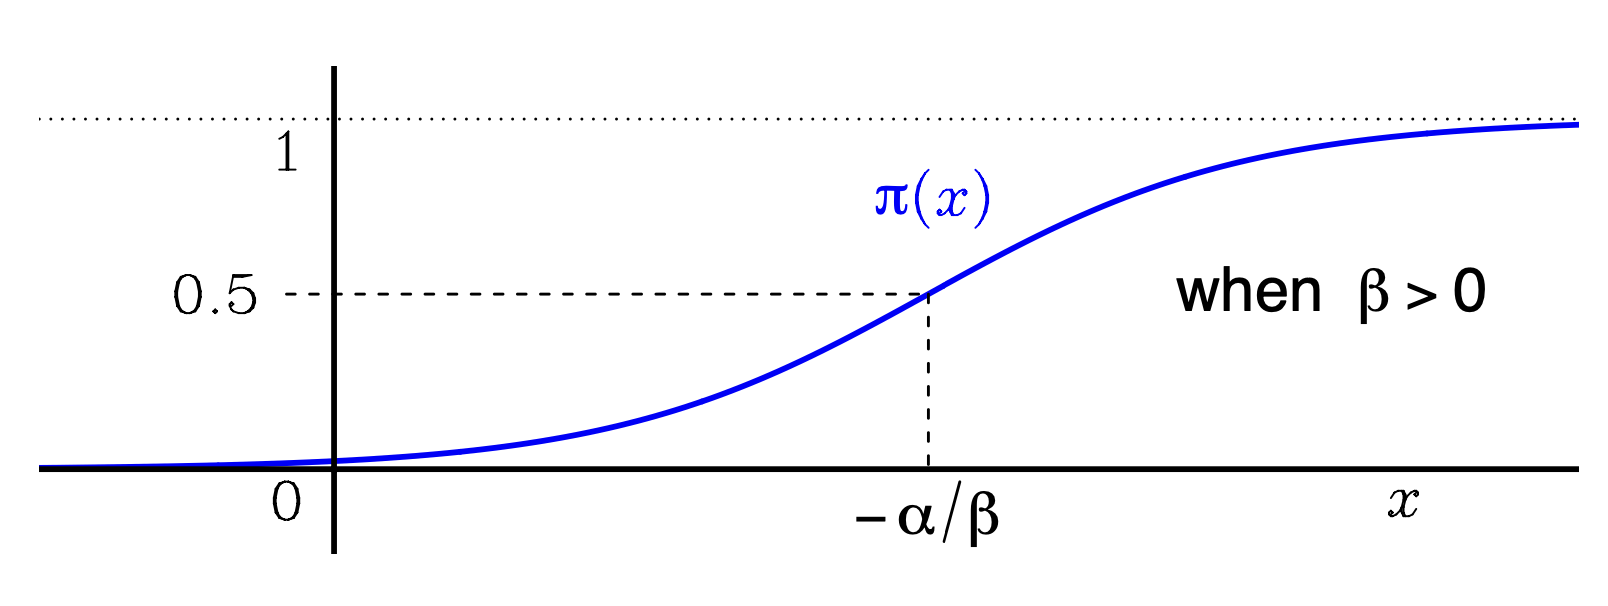
\includegraphics[scale=0.18]{logit.png}
            \caption{$\pi(x)=\frac{e^{\alpha+\beta x}}{1+e^{\alpha+\beta x}}$}
            \label{}
        \end{figure}\end{center}
    \end{enumerate}
\end{example}

\subsection{Grouped Data: Binomial Response}
If several observations have the same $\vec{x}$ ("replications"), then they have the same $\pi(\vec{x})$.

Summing binary (0/1) observations with the same $\vec{x}$ gives \textbf{grouped} data:
$$
Y_i \sim \operatorname{binomial}\left(n_i, \pi\left(\vec{x}_i\right)\right)
$$
where "$i$" now refers to the $i^{\textnormal{th}}$ group (of $n_i$ binary obs.).\\
\textit{Note}: Both $Y_i$ and $n_i$ (or $n_i-Y_i$) must be included in the data.

\textit{Remarks}:
\begin{enumerate}
    \item Whether data are grouped or ungrouped, fitting with maximum likelihood gives the same results.
    \item Technically, the binomial GLM should use $\bar{Y}_i=\frac{Y_i}{n_i}$ as the responses, and use an \textit{exponential dispersion family form} for the density.
\end{enumerate}

$$
\begin{array}{l|l|l|l}
x=1 \\
\cline { 2 - 3 } x=0 & Y_1 & n_1-Y_1 & n_1 \\
\cline { 2 - 3 } & Y_2 & n_2-Y_2 & n_2 \\
\cline { 2 - 4 } & &
\end{array}
$$
Note: Can regard as grouped data with two groups.
A binomial regression model (with $x=0$ or 1 ) is equivalent to the independent binomial model:
$$
\left.\begin{array}{l}
Y_1 \sim \operatorname{binomial}\left(n_1, \pi_1=\pi(1)\right) \\
Y_2 \sim \operatorname{binomial}\left(n_2, \pi_2=\pi(0)\right)
\end{array}\right\} \textnormal{ independent}
$$






\begin{example}[ (Poisson Regression)]
    $$
    Y_i \sim \operatorname{Poisson}\left(\mu_i\right) \quad\left(\theta_i=\mu_i\right)
    $$
    Note: $\mu_i=E\left(Y_i\right)$
    $$
    \begin{aligned}
    f\left(y_i ; \mu_i\right) & =\frac{\mu_i^{y_i}}{y_{i} !} e^{-\mu_i} \\
    & =e^{-\mu_i} \frac{1}{y_{i} !} \exp \left(y_i \ln \mu_i\right)
    \end{aligned}
    $$
    So
    $$
    \begin{gathered}
    a(\mu)=e^{-\mu} \quad b(y)=\frac{1}{y !} \\
    Q(\mu)=\ln \mu
    \end{gathered}
    $$
    The natural parameter is the log-mean.

    \textbf{Canonical link:}
    $$
    g(\mu)=Q(\mu)=\ln \mu
    $$
    which gives the \textbf{(Poisson) loglinear model}.
\end{example}


















\end{document}